\chapter{System Arquitecture}
\label{chapter:System_Arquitecture}
This chapter explains the full system arquitecture employed in this project. It will talk about all implementations, and the performance evaluation of each if possible. The focus will be on information:

Extracting information from unstructured data, using OCR engines and layout models.
Storing information with proper indexation for efficient semantic retrieval.
Employing prompt engineering techniques to enhance the consistency and accuracy of user interactions. 

\section{Optical Character Recognition Engines}
\label{sec:ocr}
Most documents in this thesis were digital-born PDFs, where text could be directly extracted with the \texttt{pdfreader} library. To ensure universal applicability of the RAG pipeline, an OCR fallback was included for cases where text was not embedded. 

OCR converts scanned PDFs or images into machine-readable text through preprocessing, segmentation, and recognition. Modern engines combine feature extraction, template matching, and contextual analysis with machine learning. Widely used options include Nougat \cite{blecher2023nougatneuralopticalunderstanding}, which preserves structure and outputs Markdown; Tesseract, an open-source tool supporting over 100 languages; and Google Vision API, a cloud-based service using deep neural networks for high accuracy.

In this thesis, Nougat is used as it is open-source and outputs Markdown, the preferred format for integration with large language models.



\section{Designing the Retrieval-Oriented Weaviate Schema in Edoclink}
\label{sec:schema}

The first step was the definition of a semantic data layer using Weaviate, integrated into the Edoclink platform. The goal was to capture the organizational logic of business documents (workflows, stages, entities, folders, and files) within a structure that supports semantic search and generative reasoning. To this end, six core classes were defined (Fluxo, Etapa, Entidade, Pasta, Ficheiro, Metadados), reflecting Edoclink’s information model. These were initially connected through cross-references, ensuring that workflows could be linked to their stages, entities to their folders, and files to their associated metadata. 

\begin{figure}[h!]
    \centering
    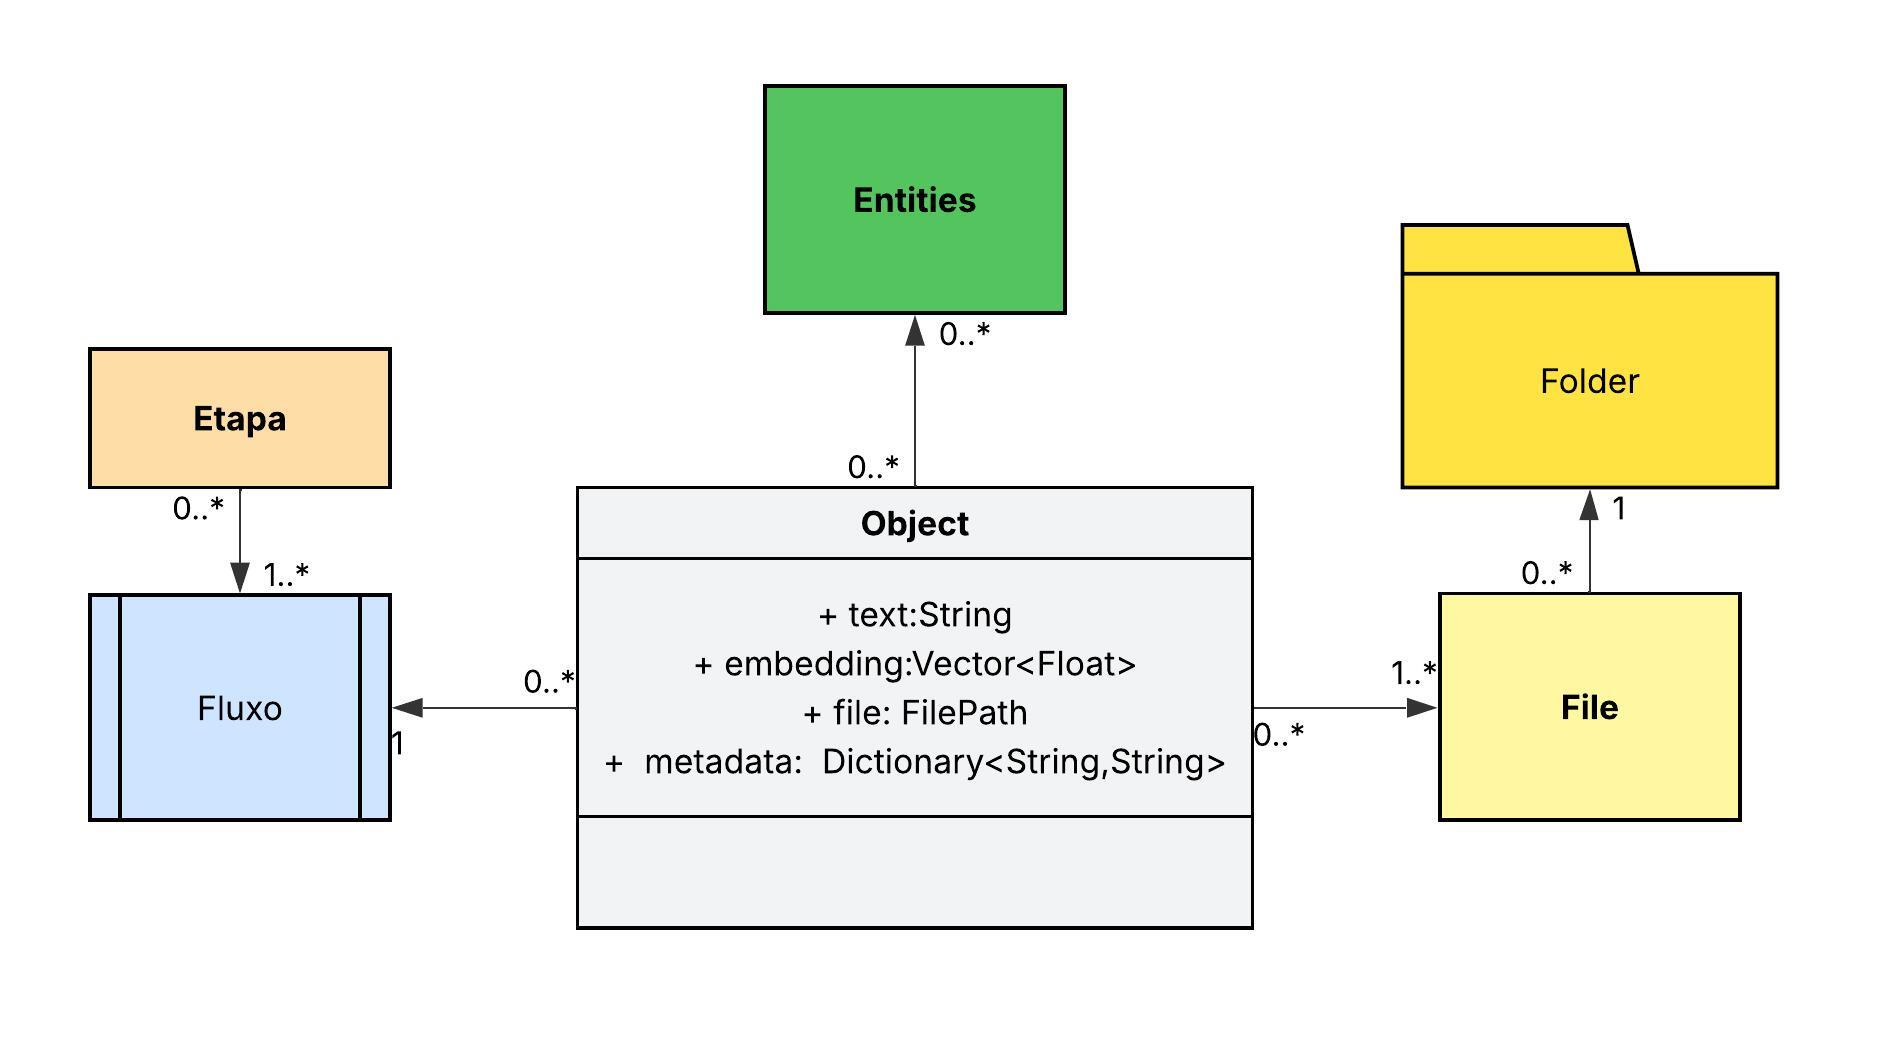
\includegraphics[width=1\linewidth]{Images/Classe UML.jpeg}
    \caption{Abstract UML representation of the schema structure, showing the relationships between objects, entities, folders, files, stages, and workflows in the Edoclink platform.}
    \label{fig:weaviate_class}
\end{figure}

The purpose for this research is to prove the possibility of semantic querying by organizational structure. A few examples were tested to a synthetically populated weaviate database with this schema, entities, stages, fluxes.

As the research progressed, the schema was refined by embedding \textit{entities}, \textit{file paths}, and \textit{metadata} directly into the object representation. This ensured that objects became self-contained, enabling consistent deletion cascades and reducing reliance on cross-reference traversal for retrieval. The UML diagram in Figure~\ref{fig:weaviate_class} illustrates this abstract model, which was investigated as a candidate for efficient implementation. 
In practice, the real deployment within Edoclink is more complex, but this abstraction served as a foundation for evaluating design choices and guiding the development of scalable semantic retrieval. The results presented here should therefore be interpreted as a conceptual example rather than a one-to-one description of the production system.

Weaviate natively supports multiple collections in the same instance, and this functionality is employed in Edoclink to store independent datasets under a shared schema, with each instance exposed through web hooks. While not a methodological focus of this work, this results in a decentralized-like architecture, as data is distributed across multiple instances. This design increases the complexity of retrieval, since agents must identify and query the appropriate web hooks when traversing datasets.  

In summary, this section has focused on the database perspective: defining the schema, refining it through embedded fields, and placing it in the context of multi-tenant storage. The next section shifts attention to Agentic AI, where the challenge is not schema design but orchestrating retrieval with agents. This transition reflects the broader research landscape, where developments such as Weaviate’s Query Agent \cite{weaviate} exemplify the move toward automated reasoning layers capable of multi-step retrieval and problem solving.

\section{Metadata Extraction with \gls{LLM} Profiling and Graph Structure}
The system implemented for metadata extraction builds upon the MiniRAG framework, adapting its core components to the task of extracting and structuring metadata from company documents.

The system follows a retrieval-augmented processing pipeline that integrates vector storage and graph-based knowledge representation.  
Documents are ingested, segmented, and processed to extract metadata, which is subsequently stored in a heterogeneous knowledge graph.  
This design enables search and reasoning based on generated metadata (entities and relationships), rather than relying solely on lexical or semantic similarity.

The architecture is composed of two main pipelines:  
(1) Document ingestion and metadata extraction, and  
(2) Knowledge graph construction and querying.

\subsection{Document Ingestion and Metadata Extraction}

\begin{itemize}
    \item \textbf{Chunking:} Documents are segmented into overlapping text chunks using sentence tokenization, ensuring that each chunk contains complete sentences and controlled overlap. This segmentation improves context preservation for downstream interactions.
    
    \item \textbf{Entity Extraction:} Using a \gls{LLM} guided by a few-shot prompt, the system identifies named entities within each chunk. Entities may represent \textit{projects, contracts, clients, departments, or financial elements}, depending on the examples and domain specificity of the few-shot configuration. Extracted entities are normalized and linked to their originating document.
    
    \item \textbf{Relationship Identification:} The system analyses co-occurrences and contextual dependencies between entities to infer semantic relationships. Relationships are derived from embedding-based proximity in the vector space.
    
    \item \textbf{Metadata Storage:} The resulting entities and relationships are stored across three complementary databases:
    \begin{itemize}
        \item a \textbf{Key-Value store} to hold raw document metadata (e.g., file path, document ID, author, date);
        \item a \textbf{Vector database} (e.g., Weaviate or NanoVector) to index embeddings of text chunks and entity descriptions;
        \item a \textbf{Knowledge graph} to capture structured relationships among entities and support relational reasoning.
    \end{itemize}
    This modular storage design allows both semantic retrieval and structured graph reasoning over the same dataset.
\end{itemize}
\begin{figure}
    \centering
    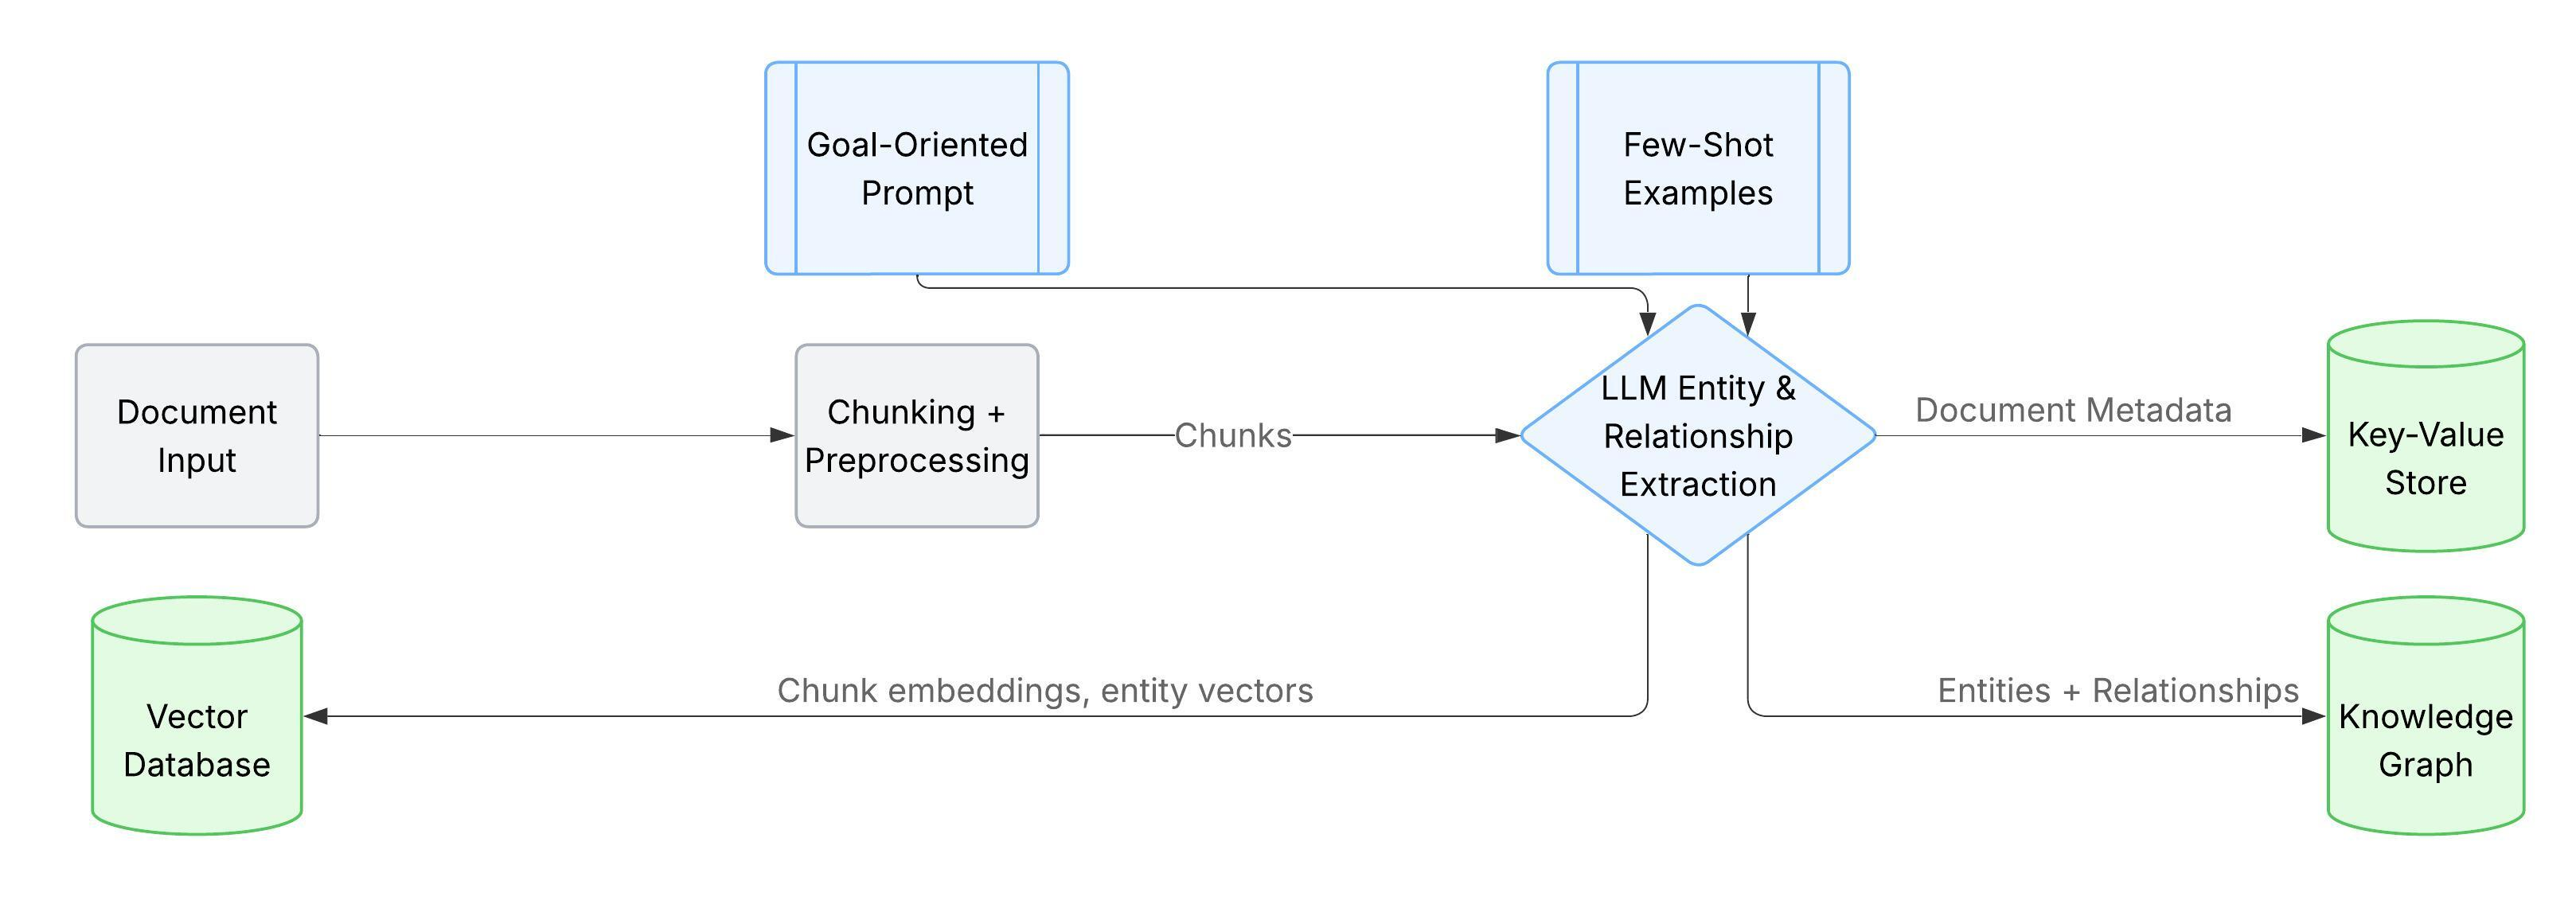
\includegraphics[width=1\linewidth]{Images/Fluxograma_Data_Processing_Pipeline.jpeg}
    \caption{Data Processing Pipeline}
    \label{fig:placeholder}
\end{figure}

\subsection{Knowledge Graph Construction}
The extracted metadata is organized into a heterogeneous graph that unifies textual, semantic, and relational information.

\begin{itemize}
    \item \textbf{Nodes} represent entities, document chunks, and other metadata fields.
    \item \textbf{Edges} represent relationships such as references, contextual links, or semantic similarity between entities.
\end{itemize}

The graph enables cross-document linking, allowing, for example, all documents referring to the same project or supplier to be discovered through relational traversal.  
It also serves as a metadata index for future retrieval tasks or RAG-based agents, grounding responses in verifiable document sources.

\begin{figure}[H]
    \centering
    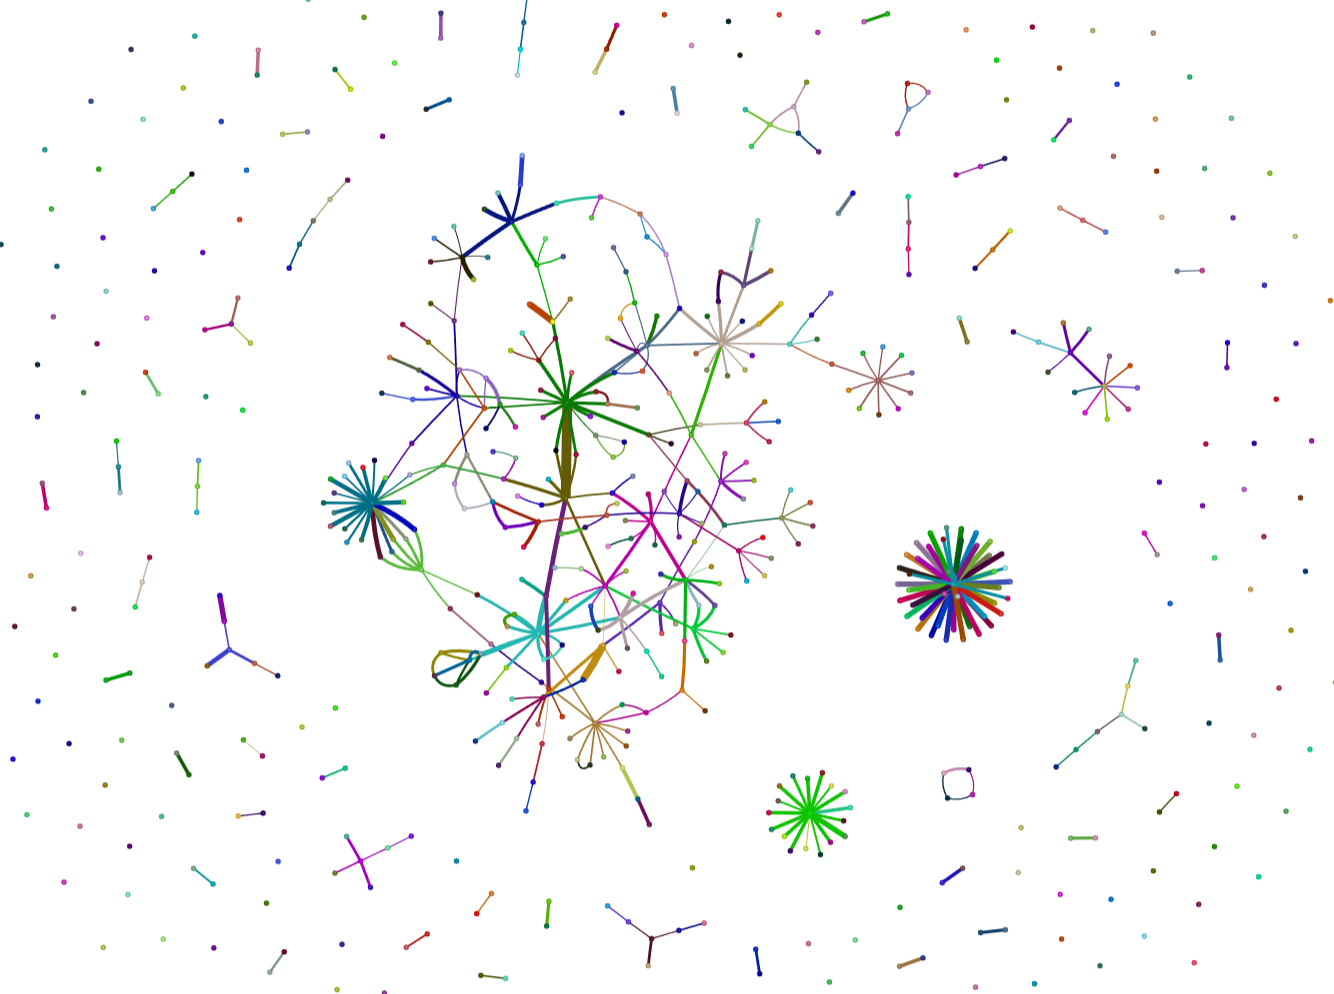
\includegraphics[width=0.5\linewidth]{Images/graph_visualisation_big.png}
    \caption{Knowledge graph from a thesis document about semantic retrieval}
    \label{fig:placeholder}
\end{figure}

\subsection{Querying}

The system supports multiple query modes (\textit{mini}, \textit{light}, \textit{naive}, \textit{doc}, \textit{meta}, \textit{BM25}, and \textit{bypass}), each offering a different retrieval strategy:
\begin{itemize}
    \item \textbf{Mini} and \textbf{Light} modes use the knowledge graph to identify entities and relationships relevant to the query, enabling context-aware retrieval.
    \item \textbf{Naive} mode performs semantic search directly over entity embeddings stored in the vector database.
    \item \textbf{Doc} mode mirrors the naive retrieval but returns the list of relevant documents instead of generating a final answer.
    \item \textbf{Meta} mode performs keyword-based search over metadata fields, implemented with autocomplete support for strict metadata queries.
    \item \textbf{BM25} mode builds a BM25 index over all chunks and retrieves text via tokenised keyword matching.
\end{itemize}
\subsection{Mini Query}

The \textit{Mini Query} mode performs multi-step reasoning over the knowledge graph to generate the most contextually accurate answer.  
It integrates keyword extraction, contextual retrieval, and answer generation into a single retrieval-augmented loop.

\begin{enumerate}
    \item \textbf{Keyword Extraction:}  
    An \gls{LLM} extracts answer-type keywords and entities from the user query using a predefined prompt (\texttt{PROMPTS["minirag\_query2kwd"]}).
    The extraction process is guided by the schema information available in the knowledge graph—specifically, the types and entities stored within it—to ensure semantic alignment between query terms and graph concepts.
    
    \item \textbf{Context Construction:}  
    Using the extracted entities and answer types, the system retrieves the corresponding nodes and relationships from the knowledge graph, as well as matching embeddings from the \gls{VD}.
    These elements are then compiled into a structured context composed of entity descriptions, related text chunks, and document snippets, forming the evidence base for the response.
    
    \item \textbf{Answer Generation:}  
    The compiled context is inserted into a response prompt (\texttt{PROMPTS["rag\_response"]}), which is passed to the \gls{LLM}.
    The model synthesizes the final answer based on the retrieved contextual evidence, ensuring that generation remains grounded in verified document content.
\end{enumerate}

\begin{figure}
    \centering
    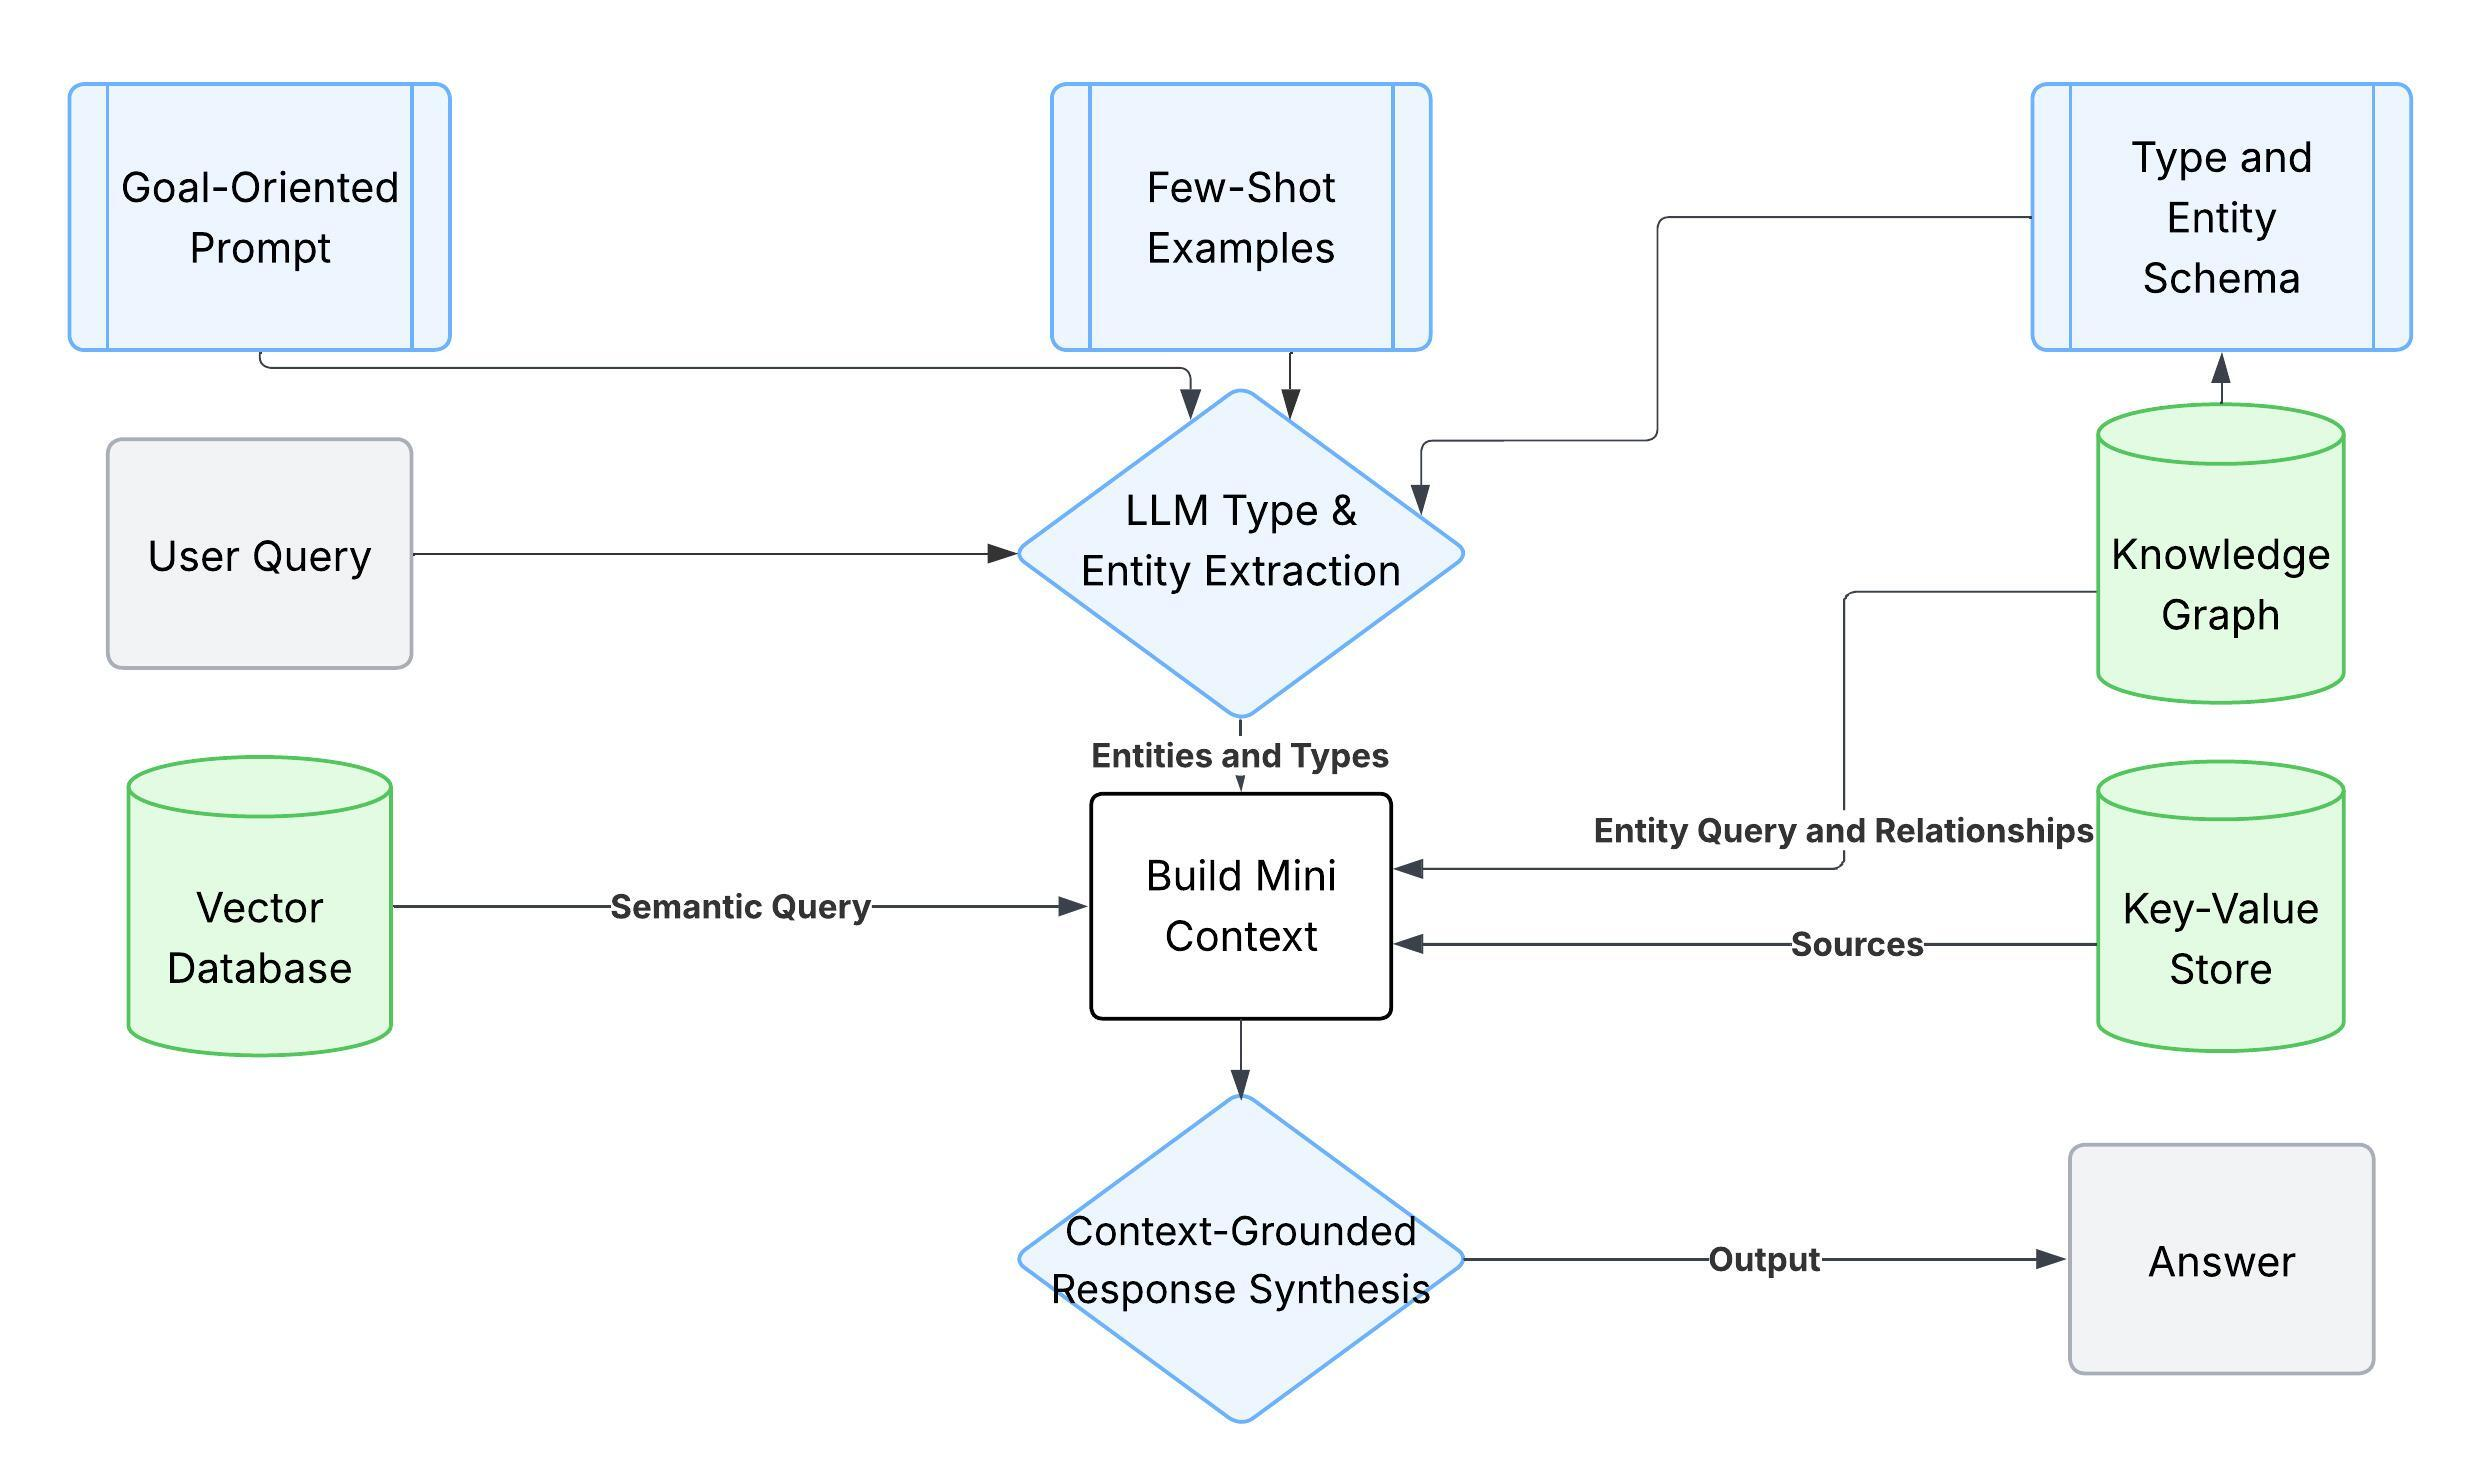
\includegraphics[width=0.75\linewidth]{Images/Fluxograma_Mini_Query.jpeg}
    \caption{Mini Query Flux}
    \label{fig:placeholder}
\end{figure}
\subsection{Summary}

In summary, the implemented system transforms unstructured corporate documents into context rich knowledge graphs by combining entity extraction, relationship identification, and graph-based storage.  
By leveraging MiniRAG’s modular retrieval and storage design, it provides a semantic layer that enriches document repositories with explicit relational metadata.  
This metadata not only supports accurate information retrieval but also enables graph-based visualization and discovery of meaningful relationships between documents, entities, and organizational processes.

\section{Weaviate MCP Server}

A \glsxtrfull{MCP} server was developed to interface with a Weaviate vector database, with the primary goal of enabling interoperability. The MCP server enables clients such as \gls{LLM}-based agents to retrieve external information from Weaviate collections in a schema-aware manner. Since Weaviate databases typically enforce a strict schema, the server provides not only query tools but also memory of the available collections and their structure. This memory is extracted from the Weaviate schema endpoint and exposed to clients as MCP resources, thereby contextualizing the agent with knowledge of valid properties before querying. When a client issues an invalid query, the server responds with an informative error listing the available fields, allowing the agent to self-correct its request automatically. The overall purpose of this server is to bridge information stored in Weaviate databases despite it's dynamic, complext and strict schemas, with powerful \gls{LLM} agents.

\subsection{Server Design}

The MCP server has been implemented in both Go and TypeScript. A Go implementation was necessary because the \texttt{mcp-registry} accepts pull requests only for Go servers; Go also offers excellent concurrency and produces lightweight binaries that can be containerized easily. If accepted, the Go version will appear in the official Docker registry, making deployment straightforward.
%% Add here a diagram showing Go server

However, the project also includes a full TypeScript implementation. This version was refactored from the original Go codebase, with additional features made possible by the improved compatibility with both the Weaviate and Anthropic SDKs \cite{stainless_mcp_comparison}. While the Go version currently supports only \texttt{stdio} transport and hybrid querying, the TypeScript implementation extends functionality with HTTP transport and native Weaviate query generation through grouped tasks. These enhancements, along with stronger documentation and tighter integration with Weaviate’s API, make the TypeScript version a more flexible and developer-friendly option while Go can be containerized easily giving better compatibilty with current \gls{MCP} registries.
%% Add here a diagram showing typescript Server
\subsection{Functionality}
The server acts as an intermediary between clients and the Weaviate backend. It registers the necessary tools and resources to support both querying and schema inspection. By exposing schema information as MCP resources (e.g., \texttt{weaviate://schema/Dataset}), the server enables clients to discover available collections and their properties (such as \texttt{targetProperties}: \{\texttt{text}: string, \texttt{filepath}: string\}). This ensures that all interactions with the database are schema-aware and self-correcting, as invalid queries are met with descriptive feedback rather than silent failures (e.g. corrective validation logic shown in figure \ref{fig:sequence-diagram-weaviate-query}). Clients are typically \gls{LLM}-powered agents capable of communicating over \gls{MCP}, allowing them to seamlessly integrate external structured knowledge into their reasoning processes.


\begin{figure}
    \centering
    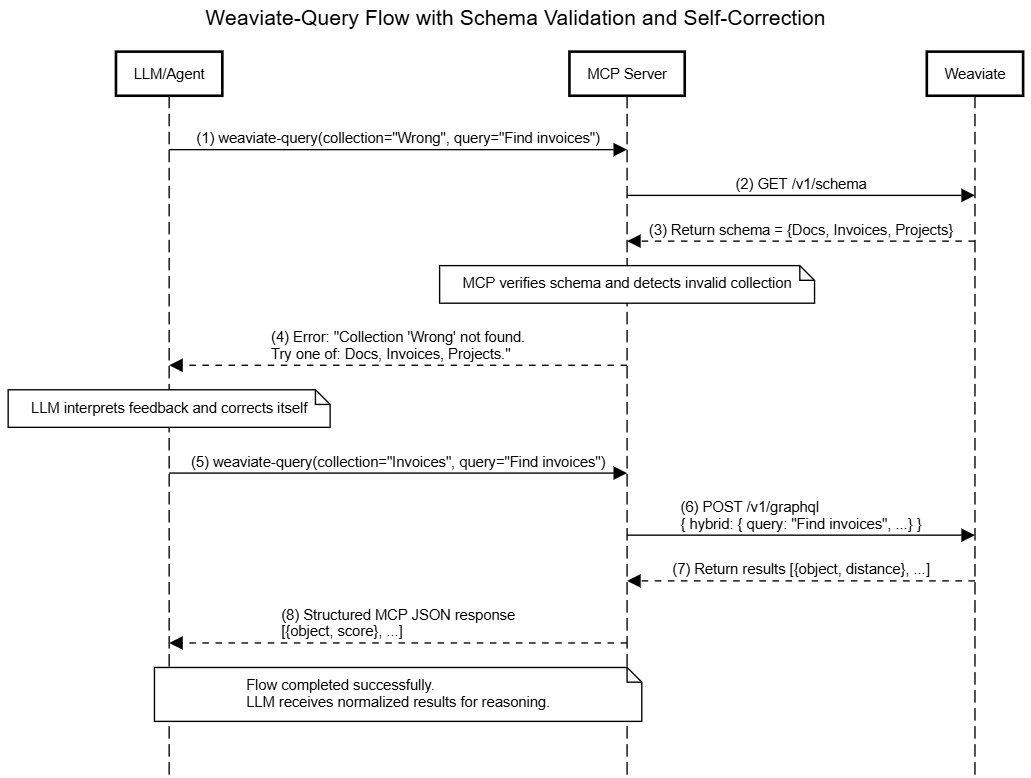
\includegraphics[width=1\linewidth]{Images/Sequence-diagram-Weaviate-Query.png}
   \caption{Sequence diagram of the \texttt{weaviate-query} tool illustrating the schema-aware approach used by the MCP Server to interface with an active Weaviate database. The same validation logic applies to other Weaviate schema elements that interface with the MCP Server.}
    \label{fig:sequence-diagram-weaviate-query}
\end{figure}






